\chapter{Simulación}
En esta sección se presentarán las simulaciones realizadas a través de LTSpiceXVII para medir los parámetros 
característicos del Darlington tanto con carga activa como carga pasiva. Por otro lado, también se desarrollará 
un análisis de Montecarlo para poder observar las sensibilidades del circuito.


\section{Circuito de Polarización}

\subsection{Carga Pasiva}

Primeramente, se realiza la simulación para la polarización del circuito con una carga pasiva de $R_E$ = $900 \Omega$.
\begin{figure}[H]
    \centering
    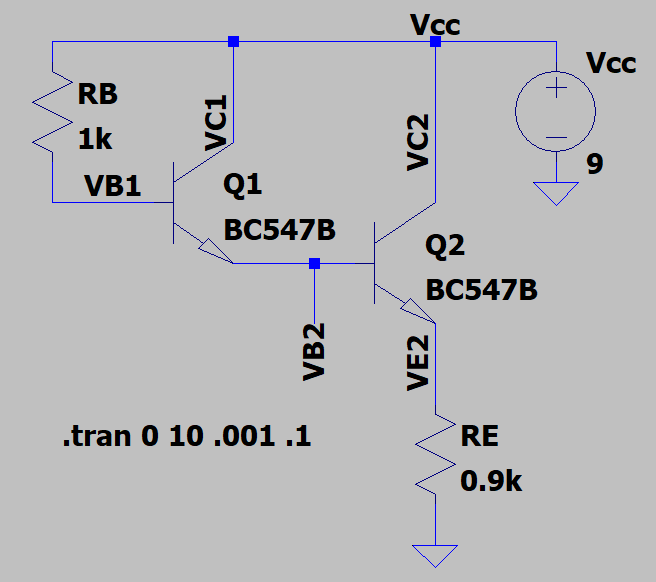
\includegraphics[width=0.5\textwidth]{3_simulacion/fig/circuito_pol_pas.png}
    \label{circuito_pol_pas}
    \caption{Circuito de Polarización configurado en LTSpiceXVII}
\end{figure}

Se obtienen los siguientes valores:

\begin{figure}[H]
    \centering
    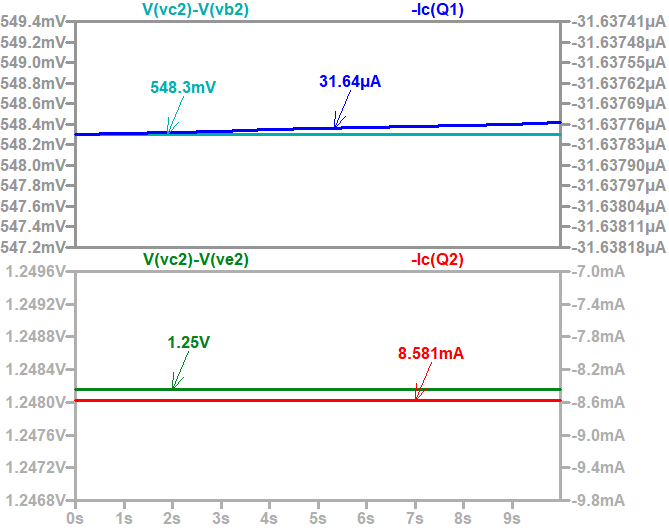
\includegraphics[width=0.75\textwidth]{3_simulacion/fig/pol_pasiva.png}
    \label{mediciones_pol_pas}
    \caption{Mediciones - Circuito de polarización con carga pasiva}
\end{figure}

A continuación se presenta una tabla con las diferencias entre el modelo teórico y simulado:

\begin{table}[H]
    \centering
    \begin{tabular}{|c|c|c|c|}
    \hline
                        & Teórico & Simulado & Error[\%] \\ \hline
    $V_{CE1}[V]$        & $0.6$   & $0.583$  & $2.9$    \\ \hline
    $V_{CE2}[V]$        & $1.2$   & $1.25$   & $4.16$   \\ \hline
    $I_{CQ1}[\mu A]$ & $29.6$  & $31.64$  & $6.89$   \\ \hline  
    $I_{CQ2}[mA]$ & $8.64$  & $8.58$  & $0.69$   \\ \hline
    \end{tabular}
    \end{table}


\subsection{Carga Activa}

Luego, se calcula  para la polarización del circuito con una carga activa implementada con un espejo de corriente.

\begin{figure}[H]
    \centering
    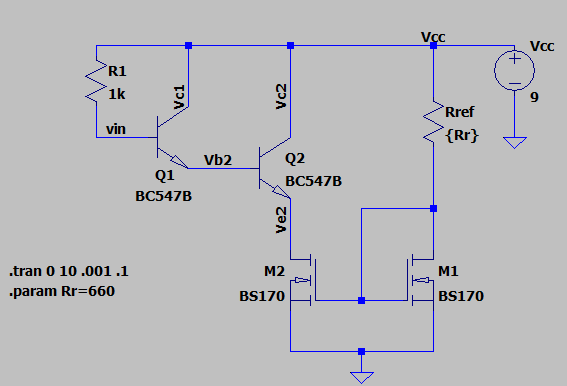
\includegraphics[width=0.5\textwidth]{3_simulacion/fig/circuito_pol_act.png}
    \label{circuito_pol_activa}
    \caption{Circuito de Polarización configurado en LTSpiceXVII}
\end{figure}

Se obtienen los siguientes valores:

\begin{figure}[H]
    \centering
    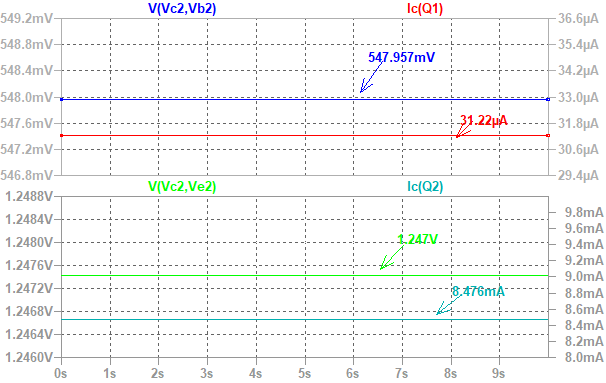
\includegraphics[width=0.75\textwidth]{3_simulacion/fig/pol_activa.png}
    \label{mediciones_pol_activa}
    \caption{Punto de operación del circuito en CC}
\end{figure}
A continuación se presenta una tabla con las diferencias entre el modelo teórico y simulado:

\begin{table}[H]
    \centering
    \begin{tabular}{|c|c|c|c|}
    \hline
                        & Teórico & Simulado & Error[\%] \\ \hline
    $V_{CE1}[V]$        & $0.6$   & $0.547$  & $9.68$    \\ \hline
    $V_{CE2}[V]$        & $1.2$   & $1.247$   & $3.91$   \\ \hline
    $I_{CQ1}[\mu A]$ & $29.6$  & $31.22$  & $5.47$   \\ \hline
    $I_{CQ2}[mA]$ & $8.64$  & $8.48$  & $1.88$   \\ \hline
    \end{tabular}
    \end{table}



\section{Parámetros de Pequeña Señal}
Lorem ipsum
\section{Circuito Incremental}
Lorem ipsum
\subsection{Ganancia de Tensión}
Para un circuito con carga pasiva se obtiene la siguiente ganancia de tensión.
\begin{figure}[H]
    \centering
    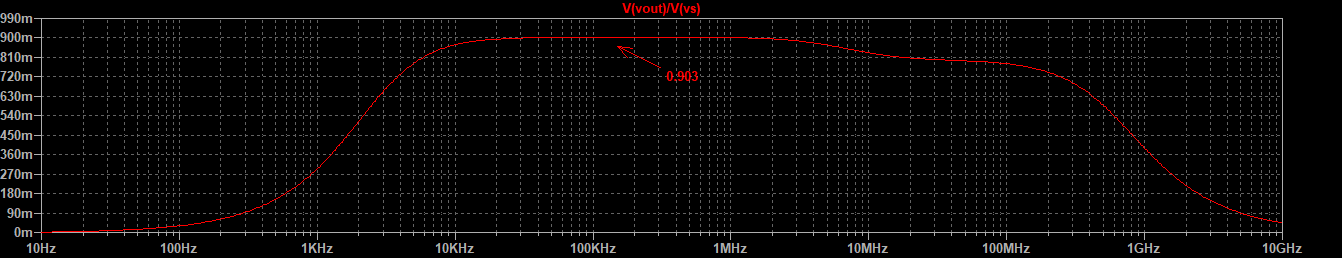
\includegraphics[width=0.75\textwidth]{3_simulacion/fig/ganancia_pasiva.png}
    \label{mediciones_pol_activa}
    \caption{Punto de operación del circuito en CC}
\end{figure}


\begin{figure}[H]
    \centering
    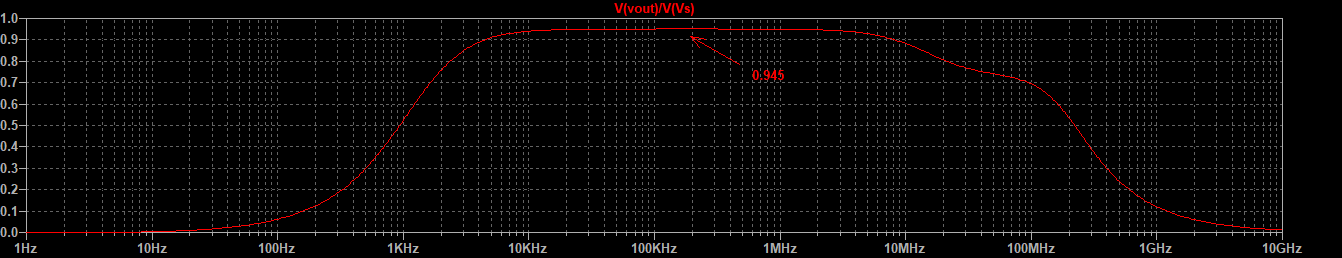
\includegraphics[width=0.75\textwidth]{3_simulacion/fig/ganancia_activa.png}
    \label{mediciones_pol_activa}
    \caption{Punto de operación del circuito en CC}
\end{figure}

\subsection{Ganancia de Corriente}

\begin{figure}[H]
    \centering
    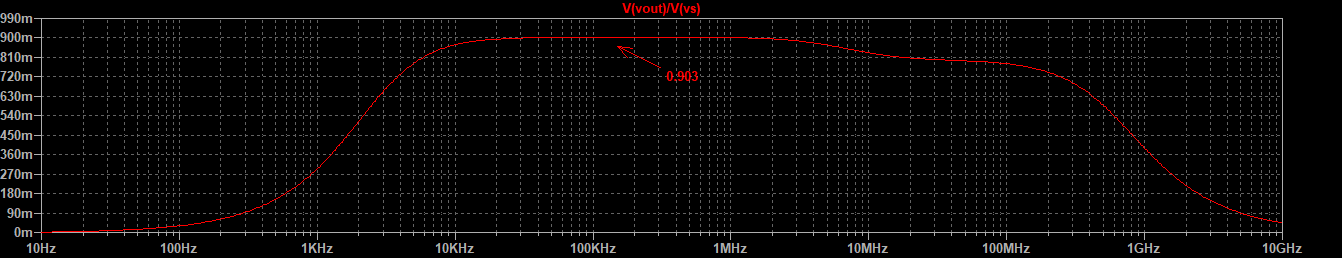
\includegraphics[width=0.75\textwidth]{3_simulacion/fig/ganancia_pasiva.png}
    \label{mediciones_pol_activa}
    \caption{Punto de operación del circuito en CC}
\end{figure}


\begin{figure}[H]
    \centering
    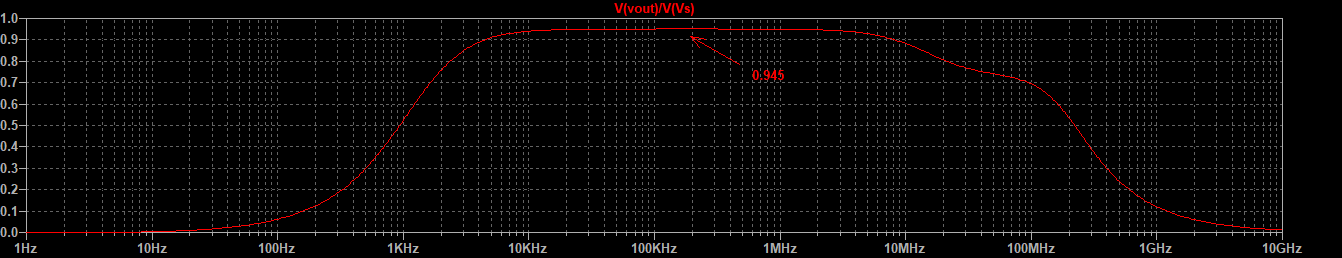
\includegraphics[width=0.75\textwidth]{3_simulacion/fig/ganancia_activa.png}
    \label{mediciones_pol_activa}
    \caption{Punto de operación del circuito en CC}
\end{figure}



\subsection{Impedancias de Entrada y Salida}
Para la impedancia de entrada se realiza la siguiente simulación:
\begin{figure}[H]
    \centering
    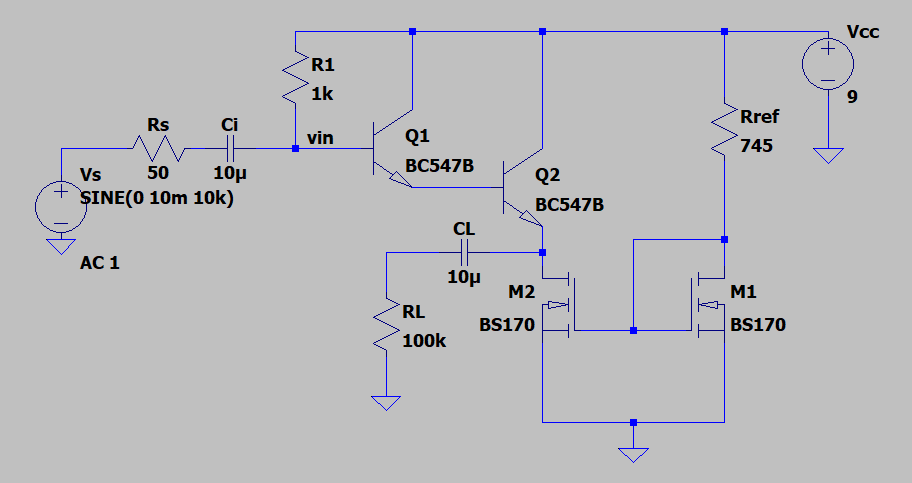
\includegraphics[width=0.75\textwidth]{3_simulacion/fig/circuito_rin.png}
    \label{mediciones_pol_activa}
    \caption{Mediciones - Circuito de polarización con carga activa}
\end{figure}
Obteniéndose los siguientes valores para la impedancia de entrada:
\begin{figure}[H]
    \centering
    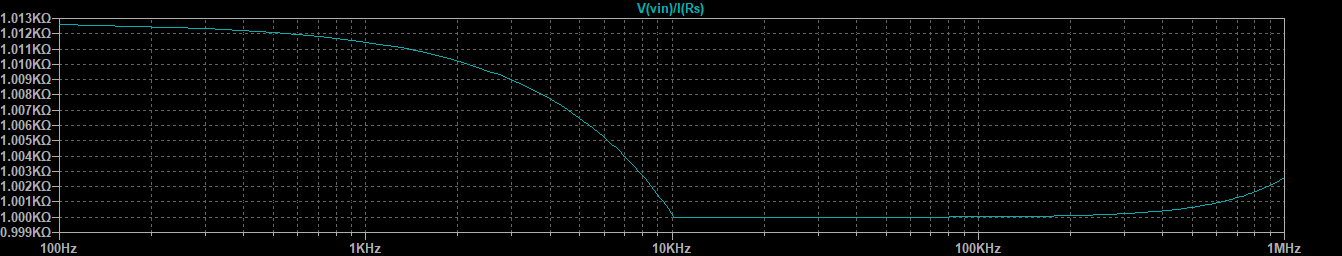
\includegraphics[width=0.75\textwidth]{3_simulacion/fig/rin.png}
    \label{mediciones_pol_activa}
    \caption{Mediciones - Circuito de polarización con carga activa}
\end{figure}

Para la impedancia de salida se realiza la siguiente simulación:
\begin{figure}[H]
    \centering
    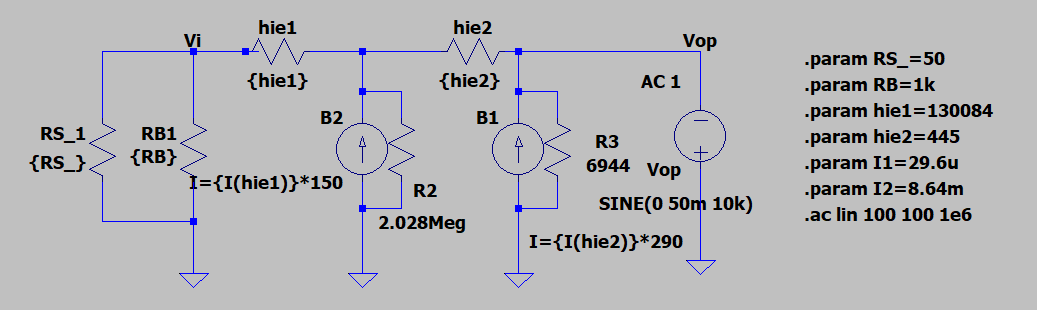
\includegraphics[width=0.75\textwidth]{3_simulacion/fig/circuito_ro.png}
    \label{mediciones_pol_activa}
    \caption{Mediciones - Circuito para medir impedancia de salida}
\end{figure}

Lorem ipsum
\subsection{Respuesta en Frecuencia}
Lorem ipsum
\newpage
\section{Circuito Incremental}
Se simuló el comportamiento del circuito incremental primero con todos los componentes y como comparación con solo el modelo de pequeña señal.

\begin{figure}[ht]
    \begin{minipage}[t]{0.45\textwidth}
        \centering
        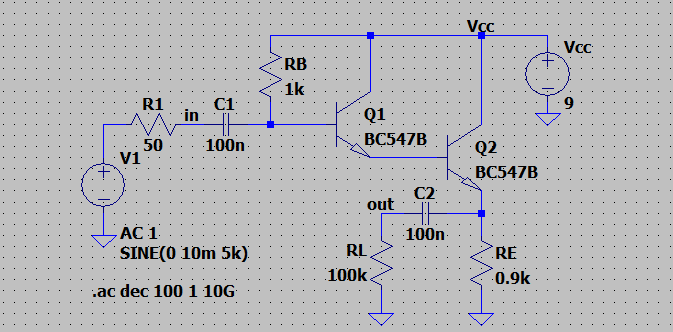
\includegraphics[width=\linewidth]{3_simulacion/fig/cir_comp_p.png}
        \caption{Circuito completo con carga pasiva}
    \end{minipage}\hfill
    \begin{minipage}[t]{0.45\textwidth}
        \centering
        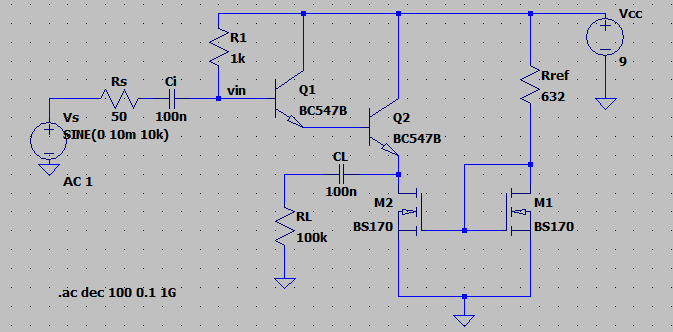
\includegraphics[width=\linewidth]{3_simulacion/fig/cir_comp_a.png}
        \caption{Circuito completo con carga activa}
    \end{minipage}
\end{figure}

\begin{figure}[ht]
    \centering
    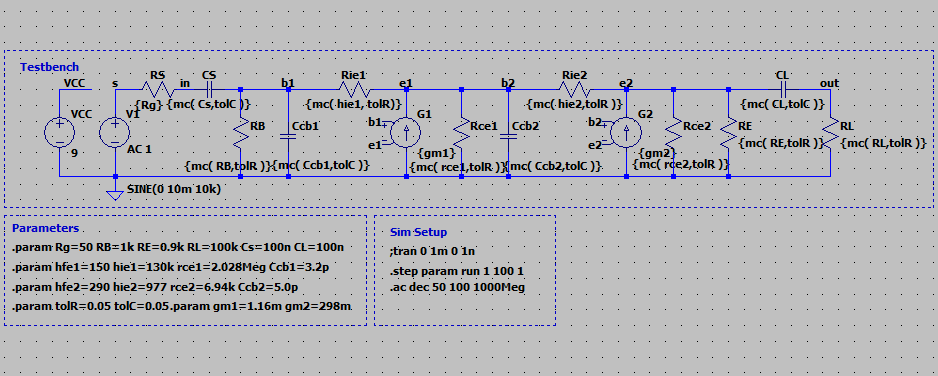
\includegraphics[width=\linewidth]{3_simulacion/fig/tb_1.png}
    \caption{Banco de prueba con modelo de pequeña señal}
\end{figure}

\begin{figure}[ht]
    \begin{minipage}[t]{0.48\textwidth}
        \centering
        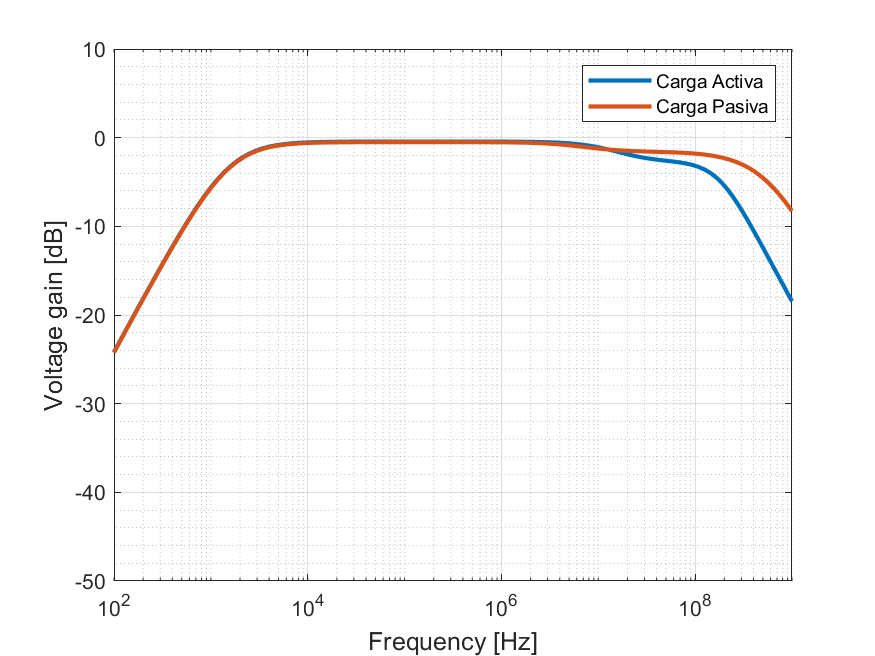
\includegraphics[width=\linewidth]{3_simulacion/fig/Bode_circuito.png}
        \caption{Respuesta en frecuencia de la ganancia de tensión de los circuitos}
        \label{fig:bode_cir}
    \end{minipage}\hfill
    \begin{minipage}[t]{0.48\textwidth}
        \centering
        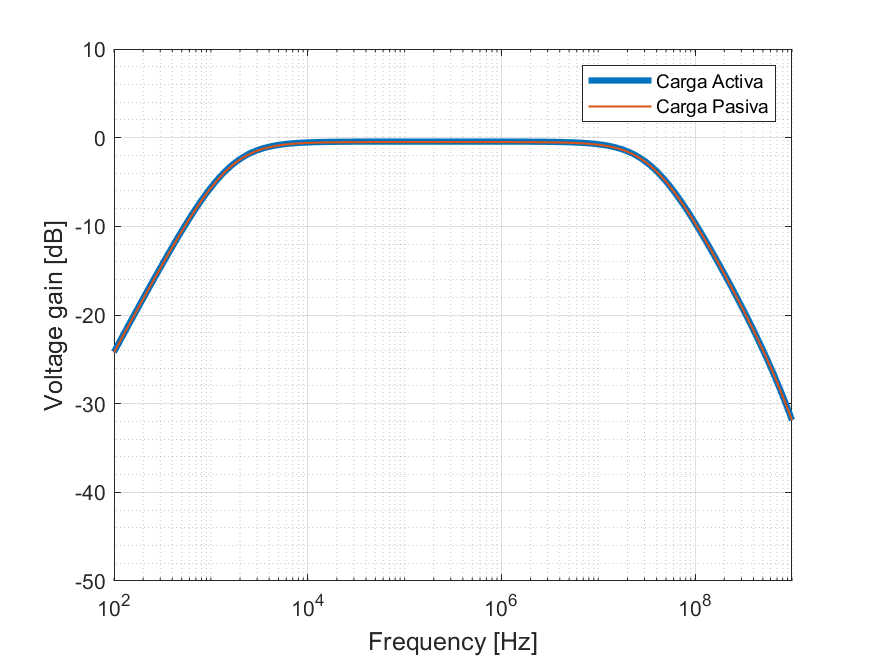
\includegraphics[width=\linewidth]{3_simulacion/fig/Bode_tb1.png}
        \caption{Respuesta en frecuencia de la ganancia de tensión del banco de prueba}
        \label{fig:bode_tb1}
    \end{minipage}
\end{figure}

Se puede observar una mejora en el circuito con carga activa al acortar el ancho de banda a altas frecuencias en la figura \ref{fig:bode_cir}. Por otro lado, hay una diferencia considerable entre la respuesta en frecuencia del circuito real y la del modelo incremental. Se encontró que esto ocurre por despreciar las capacitancias parásitas entre la base y el emisor.

Utilizando una nueva configuración donde se consideraron estas capacitancias, se obtuvo una simulación más acorde a la del circuito real (figura \ref{fig:bode_tb2}). Aún así, el circuito conserva su comportamiento de seguidor por emisor en las frecuencias medias.

Por último también se ejecutó el análisis de montecarlo para cada variación de los circuitos simulados. Se puede observar en cada caso cómo la aplicación de la carga activa en primer lugar acerca el polo dominante de alta frecuencia, reduciendo el ancho de banda.

\begin{figure}
    \centering
    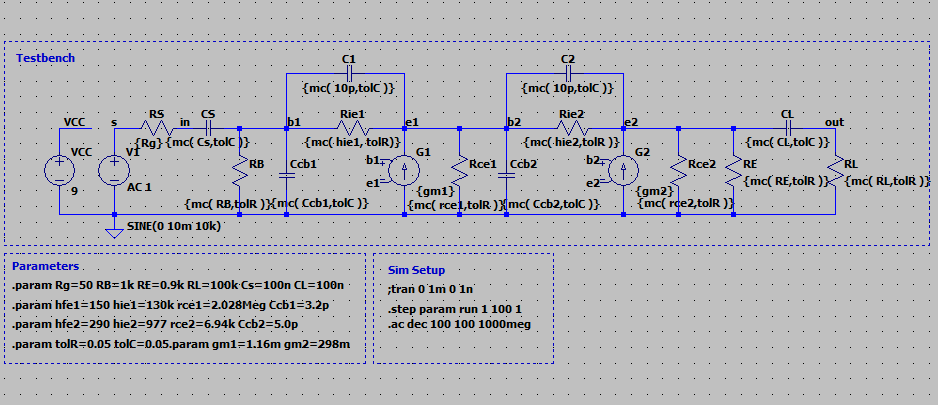
\includegraphics[width=\linewidth]{3_simulacion/fig/tb_2.png}
    \caption{Banco de pruebas con Capacitancias Base Emisor}
\end{figure}

\begin{figure}
    \centering
    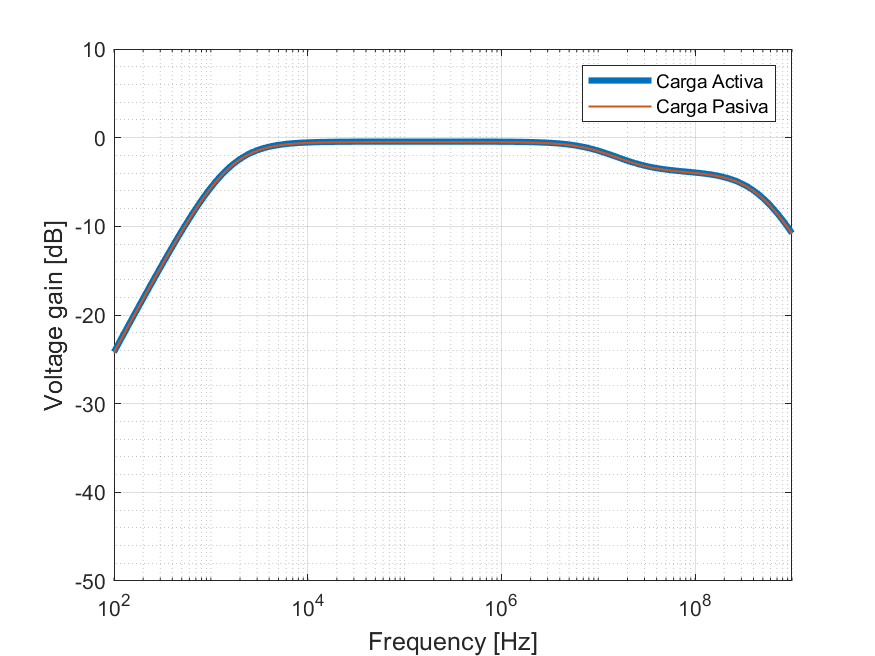
\includegraphics[width=0.5\linewidth]{3_simulacion/fig/Bode_tb2.png}
    \caption{Respuesta en frecuencia del banco de prueba con $C_{eb}$}
    \label{fig:bode_tb2}
\end{figure}

\begin{figure}
    \centering
    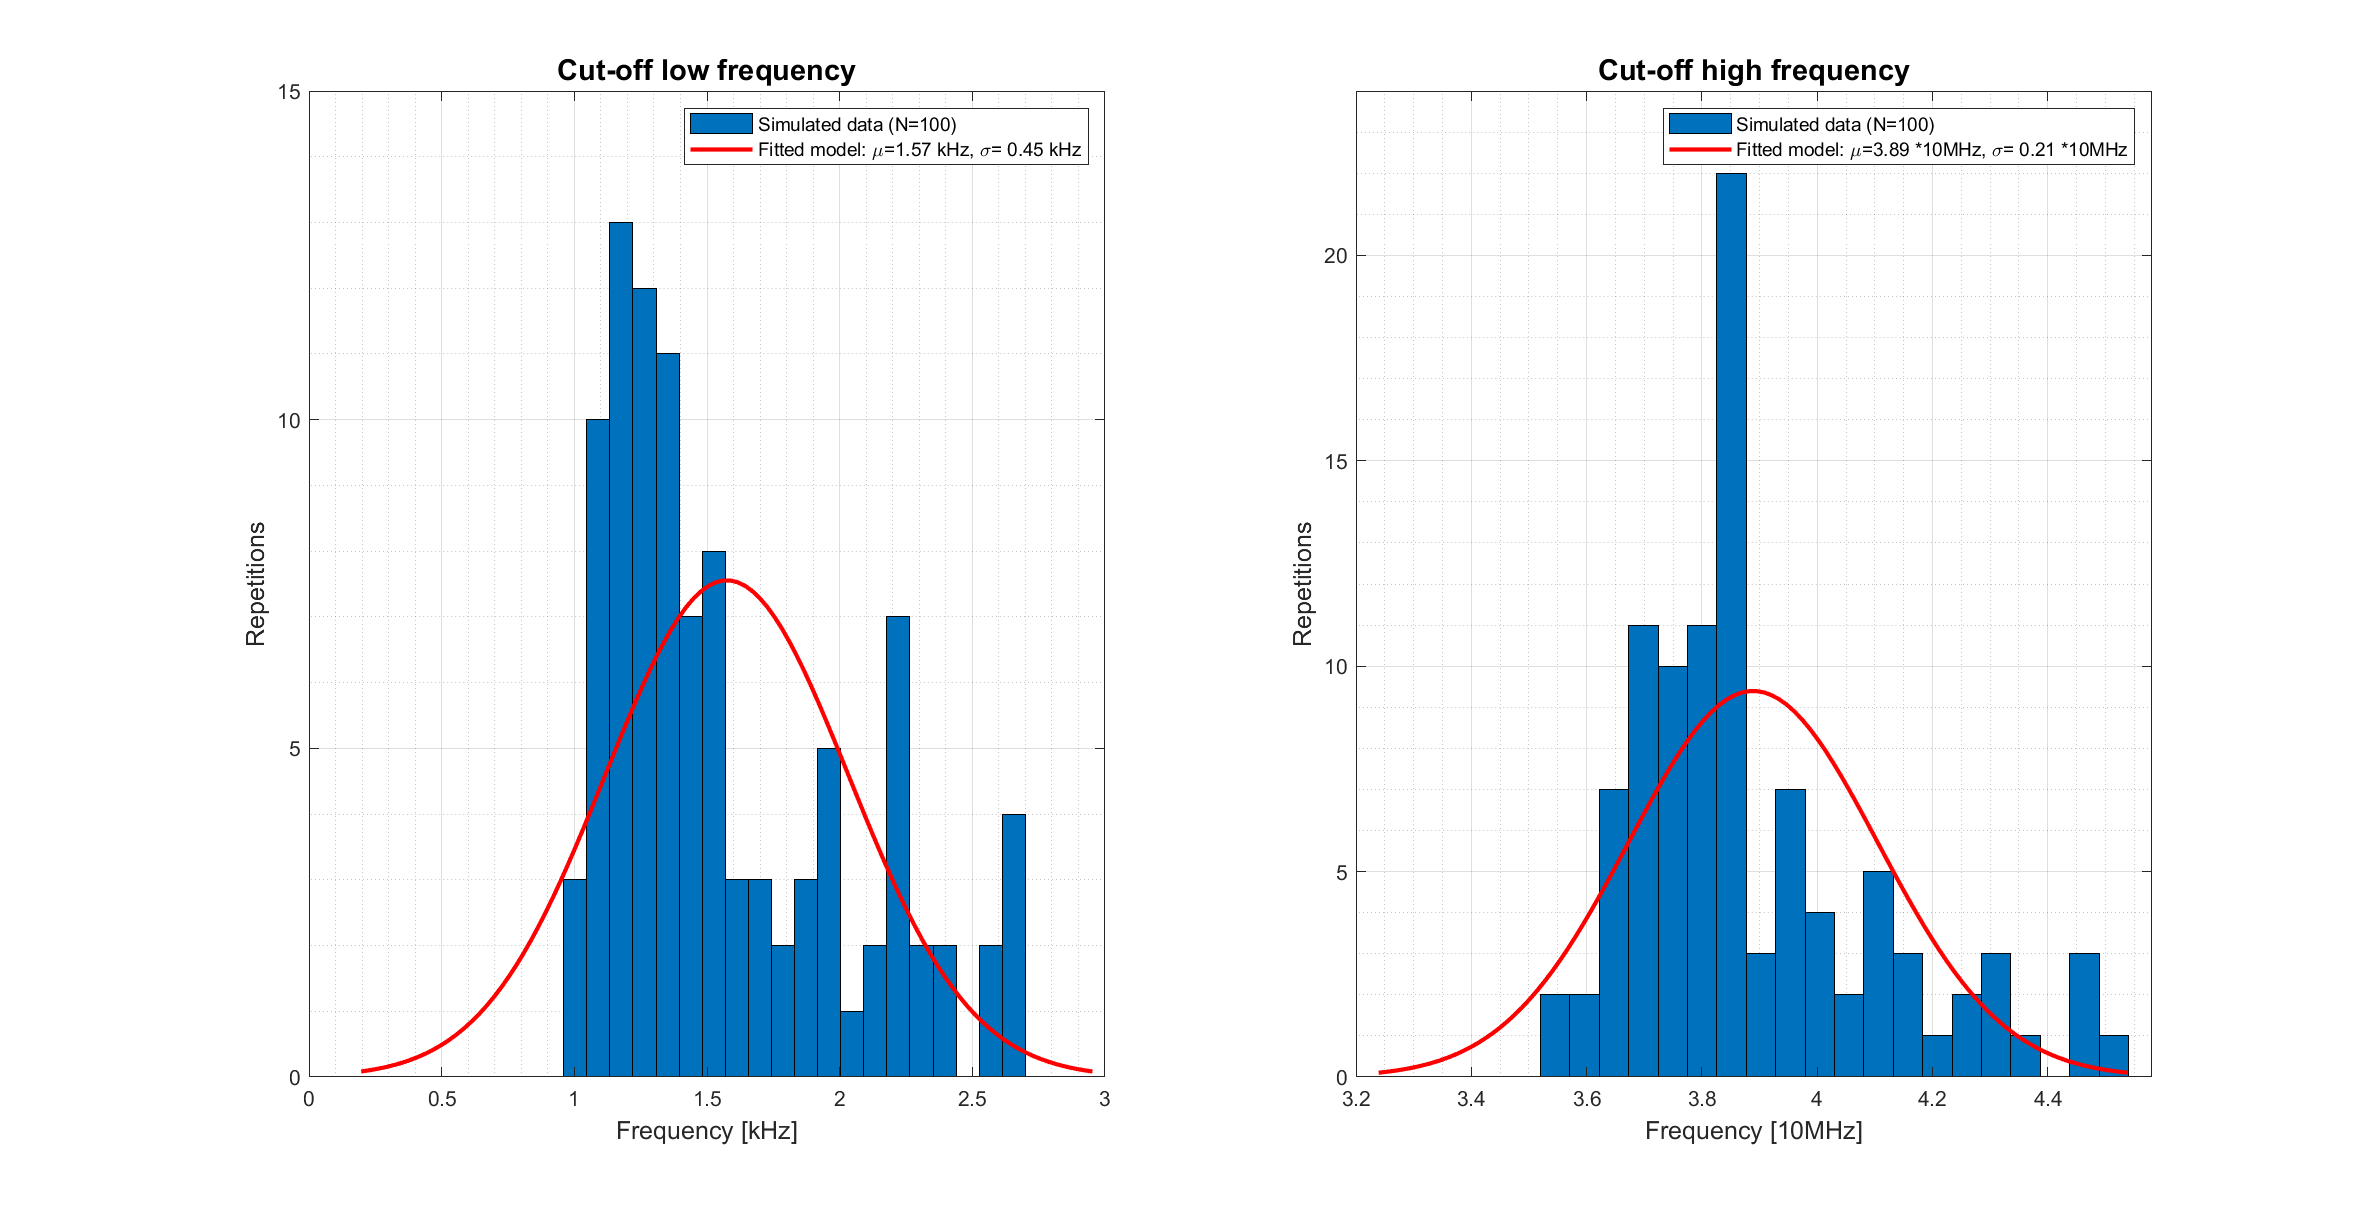
\includegraphics[width=\linewidth]{3_simulacion/fig/Hist_cir_pas_100.png}
    \caption{Análisis estadístico de los lugares de los polos de bajas y altas frecuencias con carga pasiva, circuito real}
\end{figure}

\begin{figure}
    \centering
    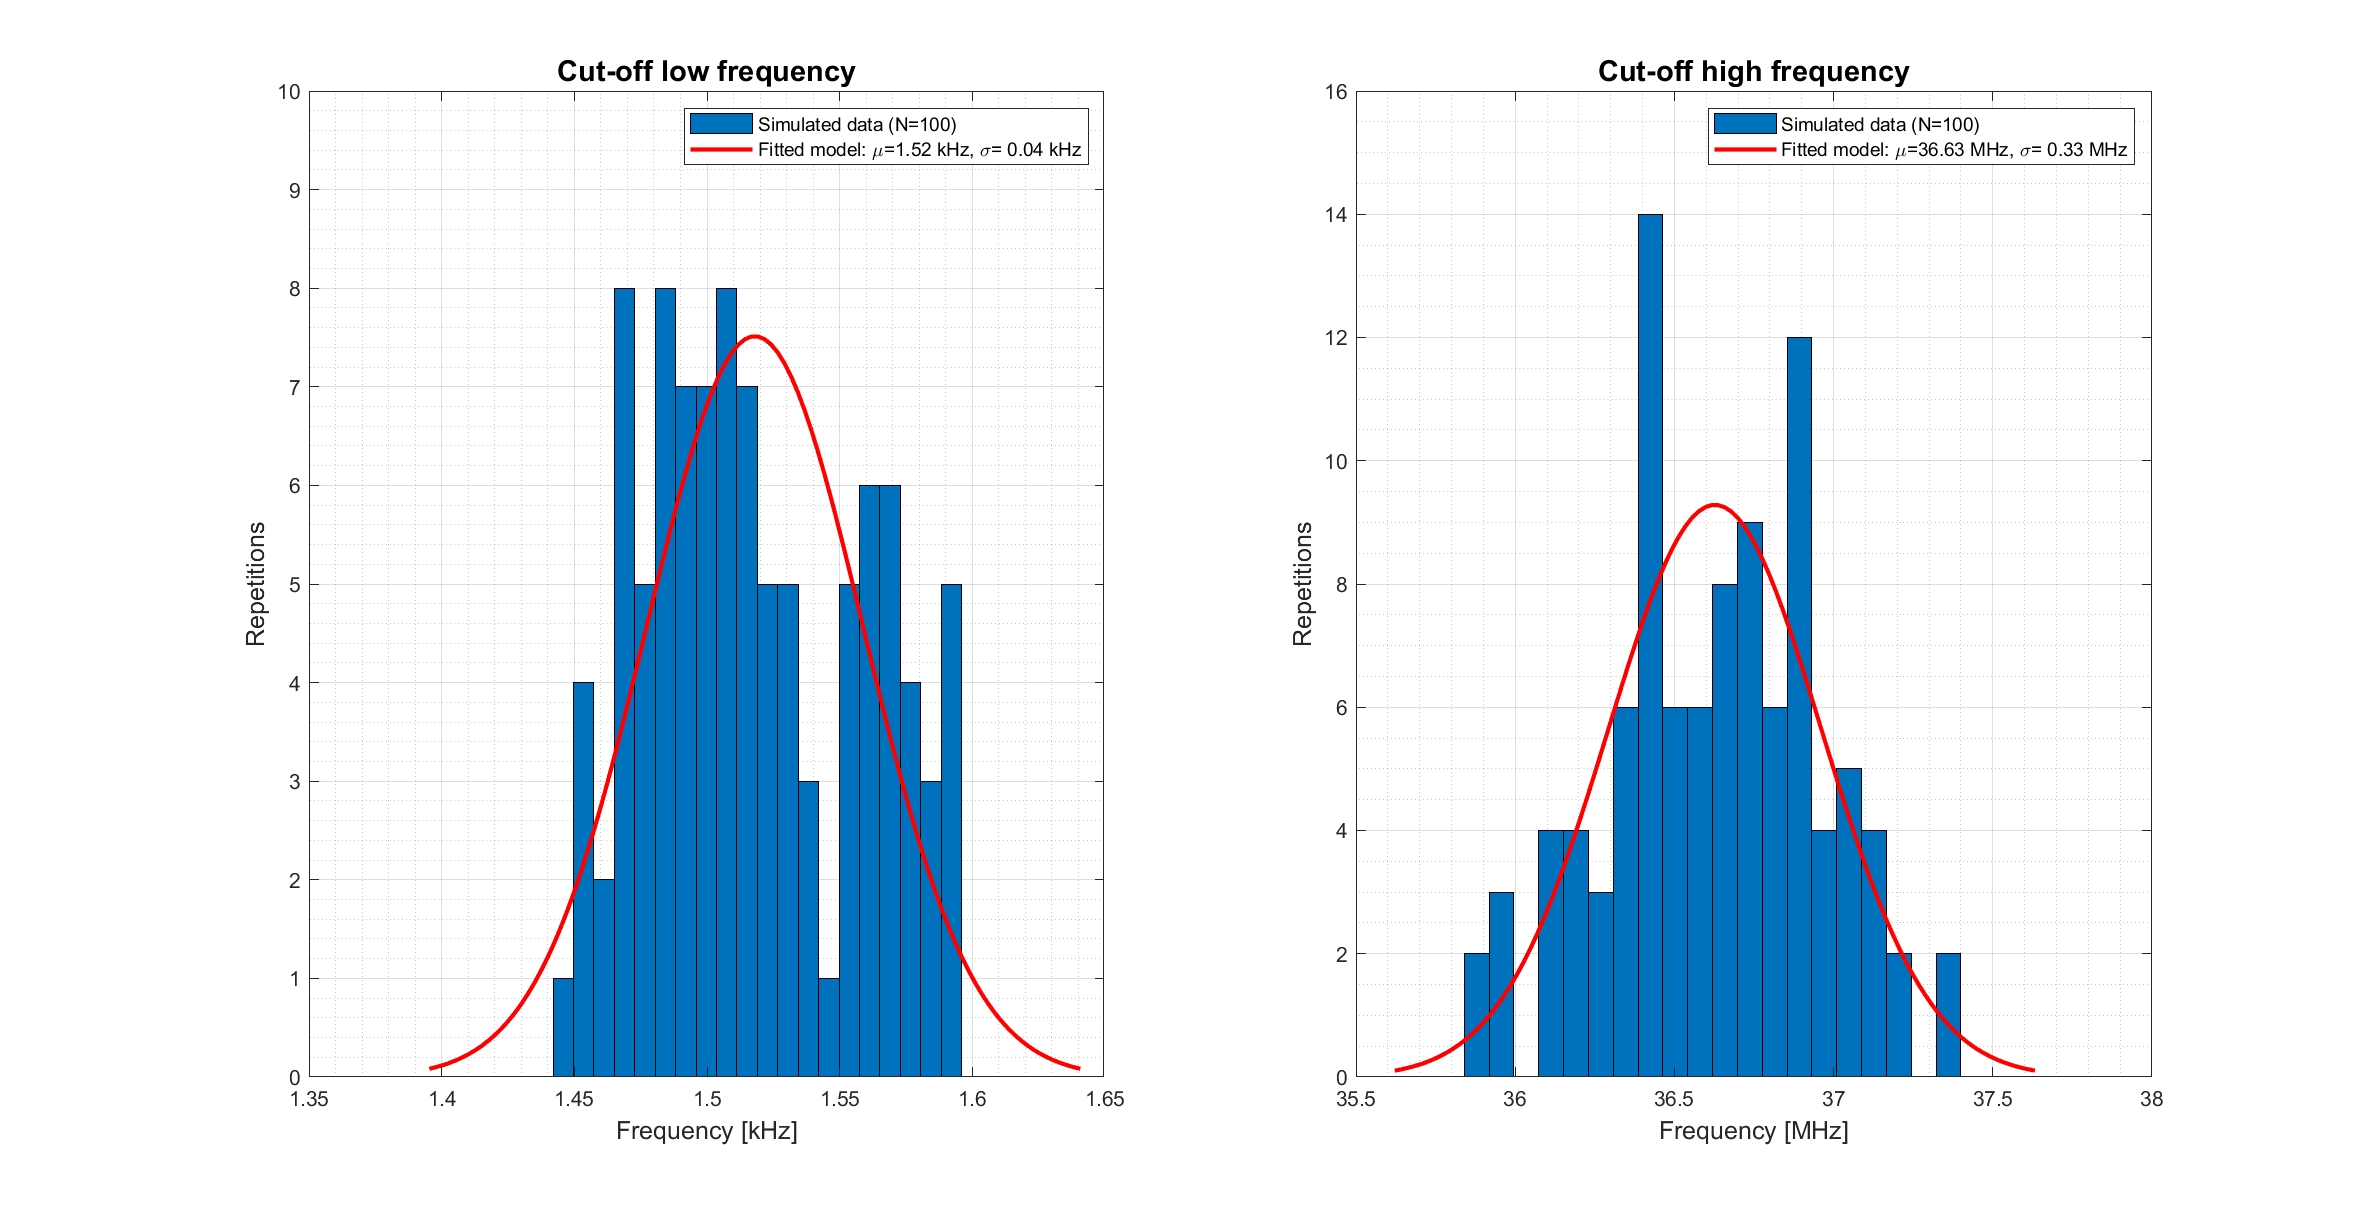
\includegraphics[width=\linewidth]{3_simulacion/fig/Hist_cir_act_100.png}
    \caption{Análisis estadístico de los lugares de los polos de bajas y altas frecuencias con carga activa, circuito real}
\end{figure}

\begin{figure}
    \centering
    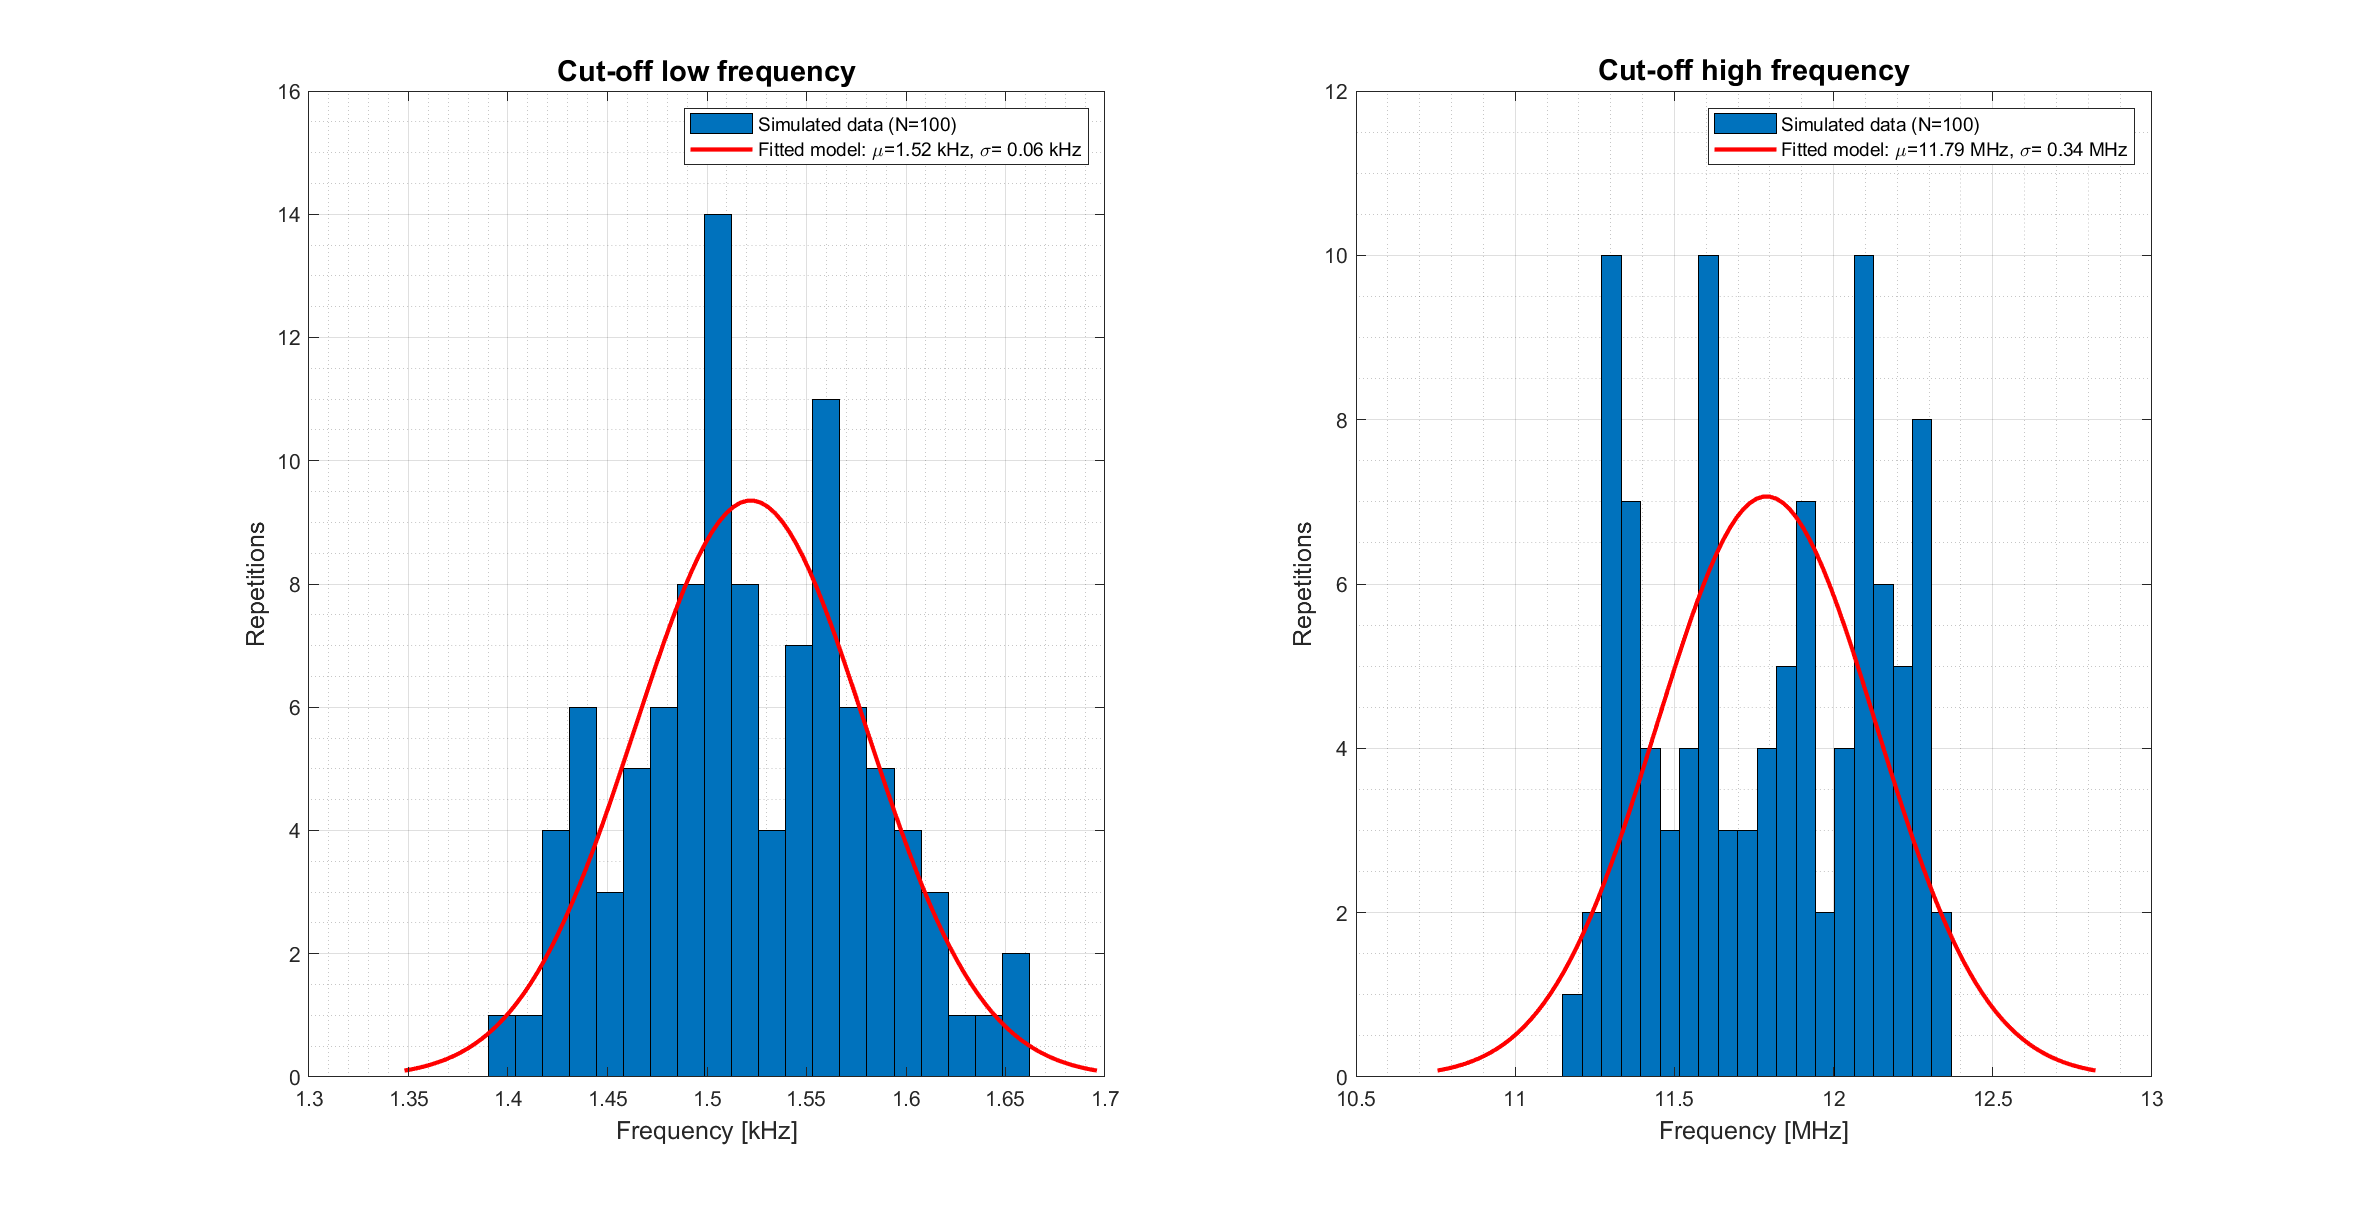
\includegraphics[width=\linewidth]{3_simulacion/fig/Hist_tb1_pas_100.png}
    \caption{Análisis estadístico de los lugares de los polos de bajas y altas frecuencias con carga pasiva, banco de pruebas 1}
\end{figure}

\begin{figure}
    \centering
    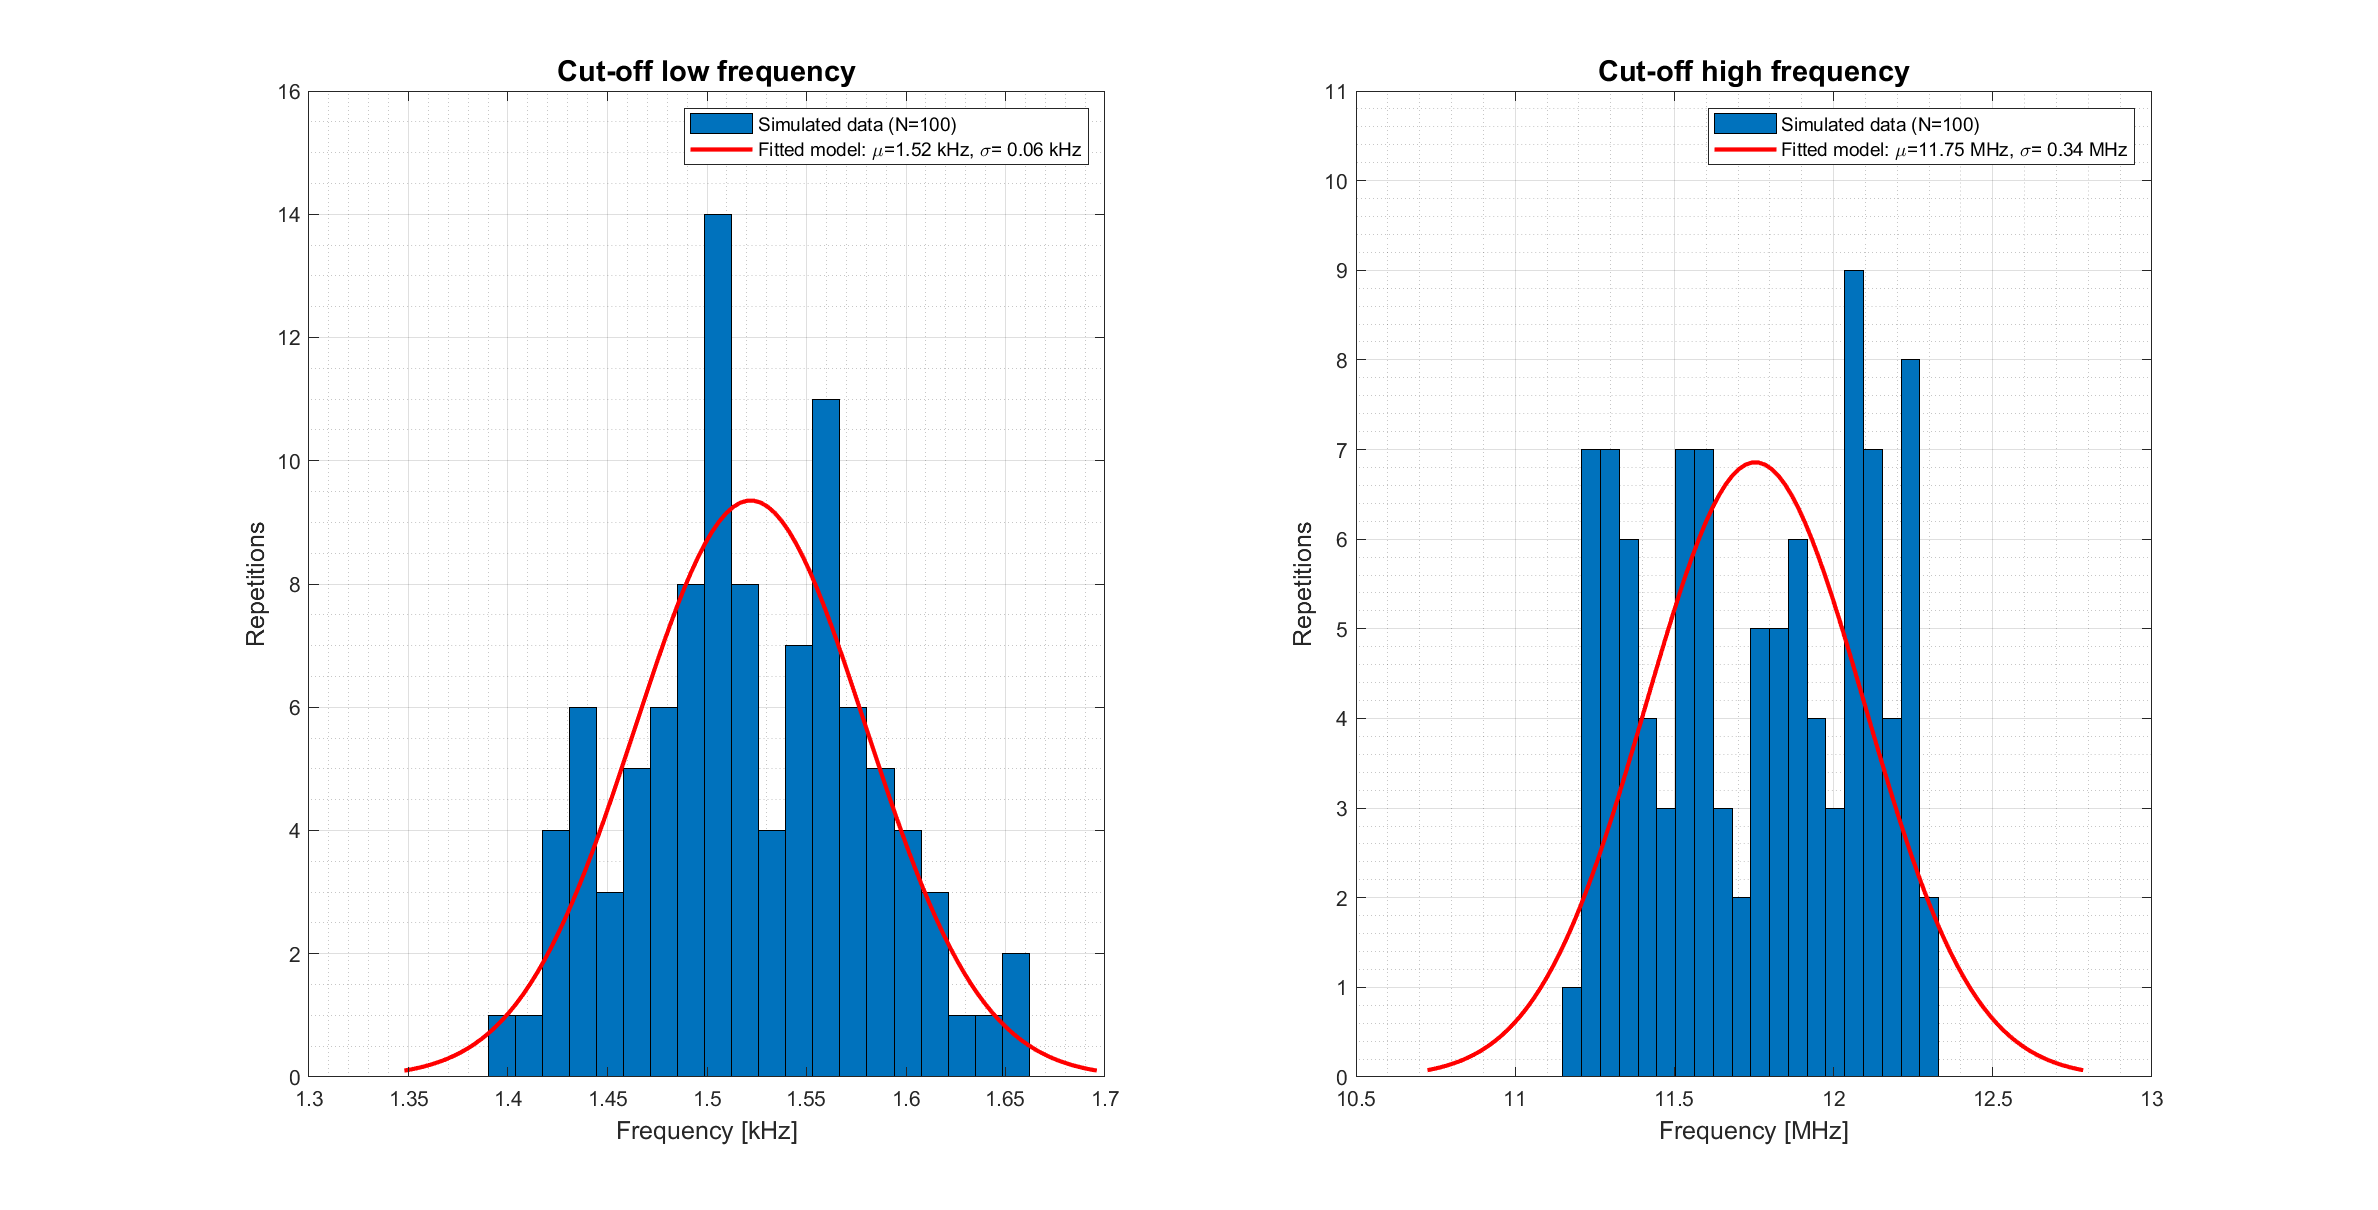
\includegraphics[width=\linewidth]{3_simulacion/fig/Hist_tb1_act_100.png}
    \caption{Análisis estadístico de los lugares de los polos de bajas y altas frecuencias con carga activa, banco de pruebas 1}
\end{figure}

\begin{figure}
    \centering
    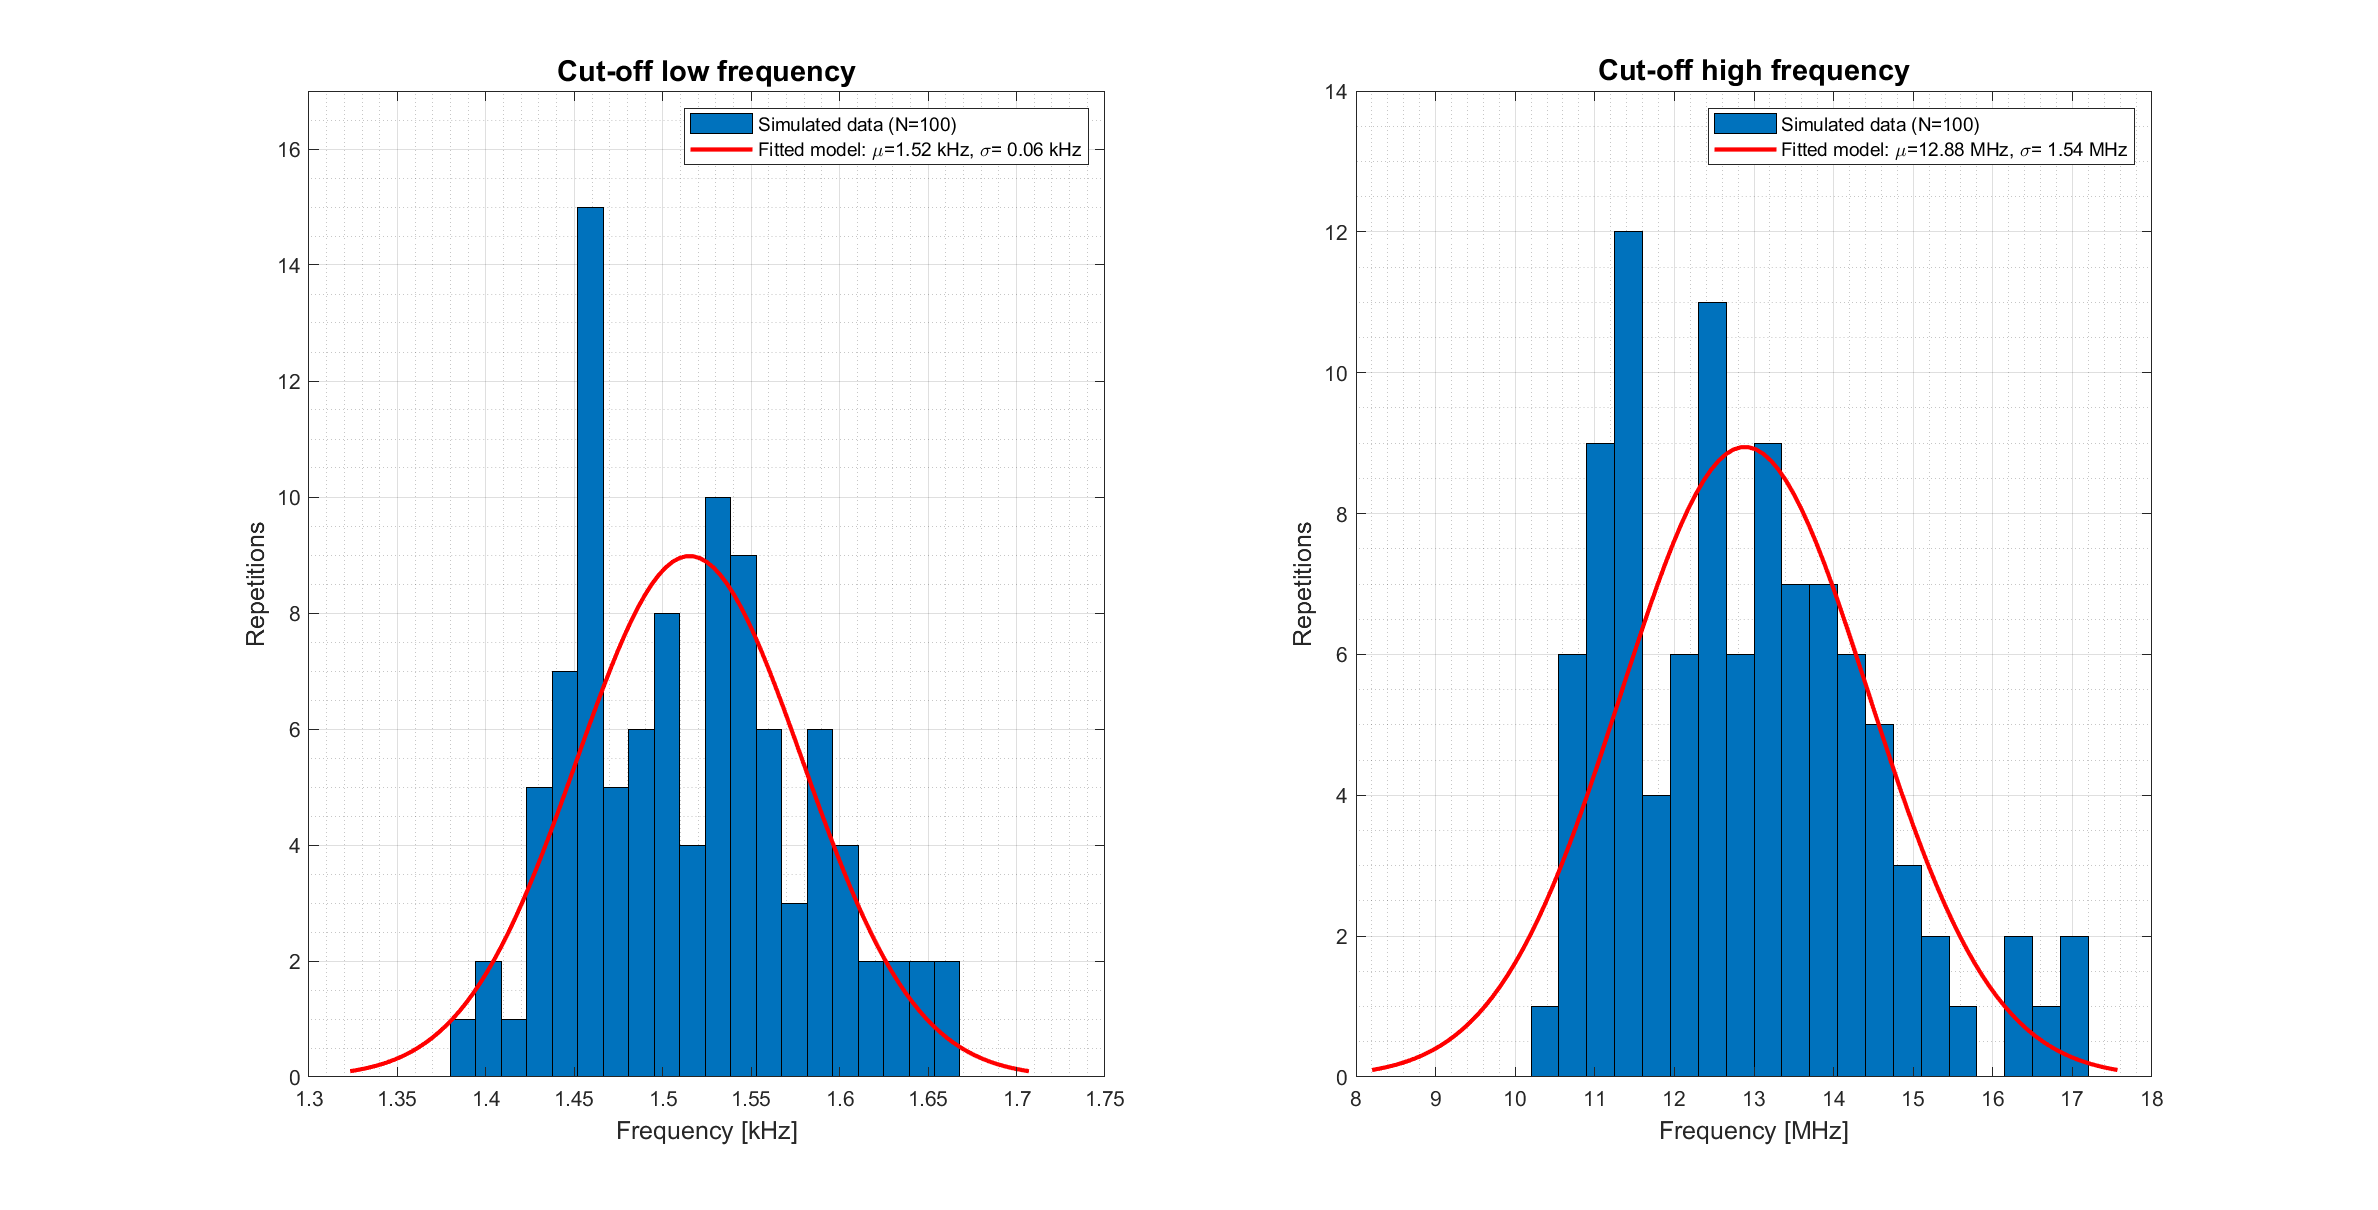
\includegraphics[width=\linewidth]{3_simulacion/fig/Hist_tb2_pas_100.png}
    \caption{Análisis estadístico de los lugares de los polos de bajas y altas frecuencias con carga pasiva, banco de pruebas 2}
\end{figure}

\begin{figure}
    \centering
    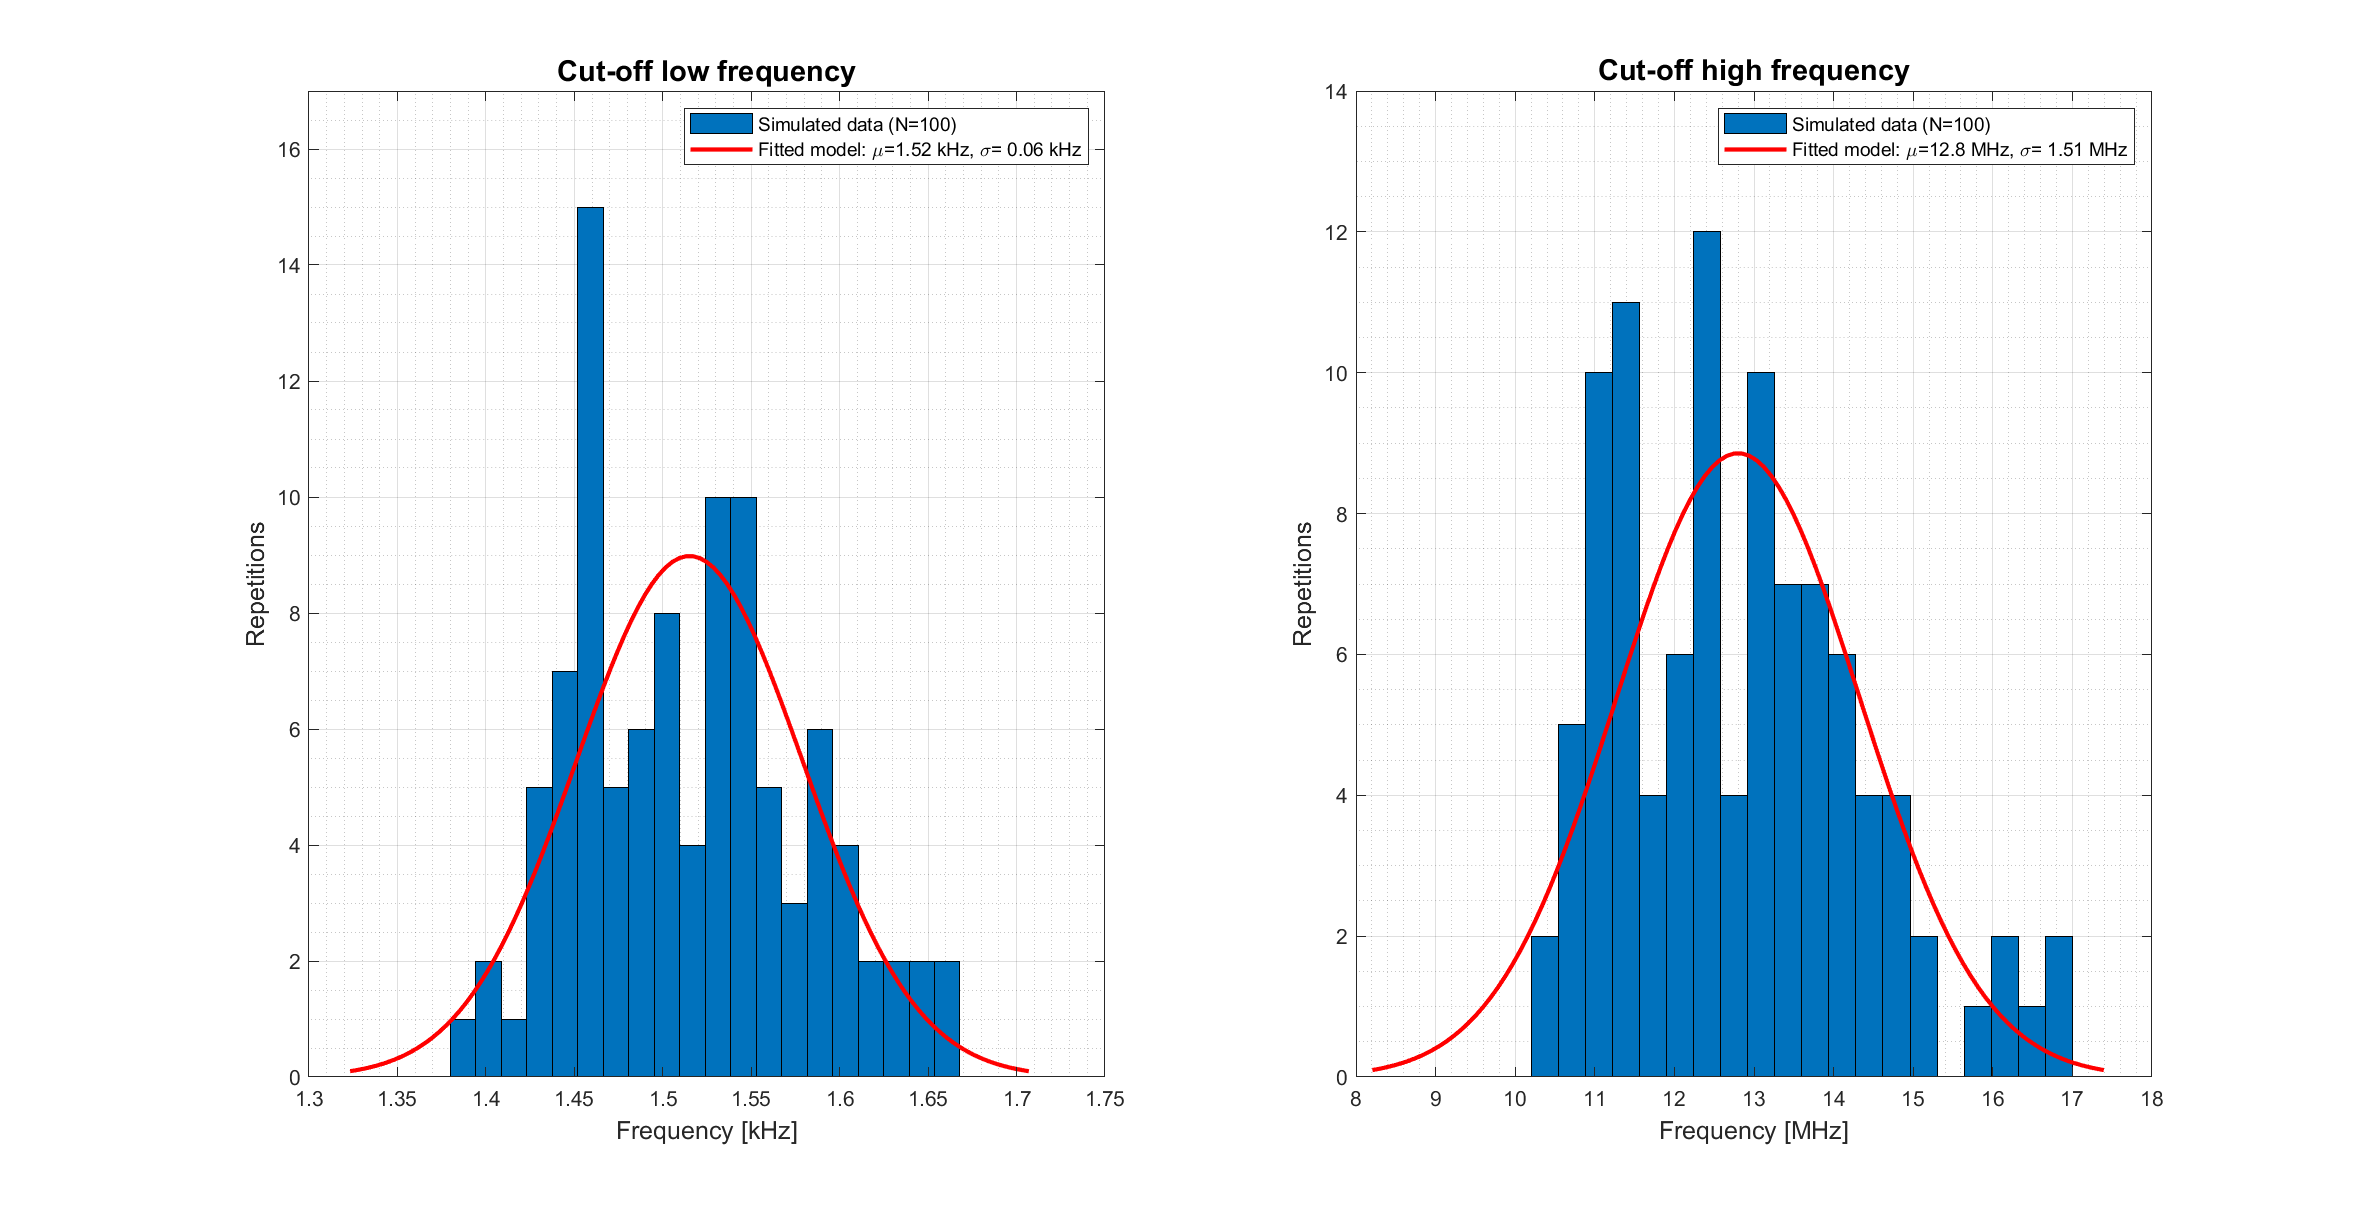
\includegraphics[width=\linewidth]{3_simulacion/fig/Hist_tb2_act_100.png}
    \caption{Análisis estadístico de los lugares de los polos de bajas y altas frecuencias con carga activa, banco de pruebas 2}
\end{figure}
